
%%
%%  Copyright 2010 Carsten Clauss, Stefan Lankes, Thomas Bemmerl
%%                 Chair for Operating Systems, RWTH Aachen University
%%

\documentclass[fontsize=10pt, paper=a4, DIV12, pagesize=auto]{scrartcl}
%\usepackage[scaled=0.92]{helvet}
\usepackage[english]{babel}
\usepackage[left]{eurosym}
%\usepackage[dvips]{hyperref}
%\usepackage[dvips]{graphicx}       % to include PS pictures 
\usepackage{hyperref}
\usepackage{graphicx} 

% set properties of PDF document
\hypersetup{colorlinks,
            linkcolor=black,
            filecolor=black,
            urlcolor=black,
            citecolor=black,
            bookmarksnumbered=true,
            pdfstartpage={1},
            pdftitle={iRCCE: A Non-blocking Communication Extension to the RCCE Communication Library for the Intel Single-Chip Cloud Computer},
            pdfsubject={API Manual},
            pdfauthor={Carsten Clauss, Stefan Lankes, Jacek Galowicz, Thomas Bemmerl},
            pdfkeywords={RCCE, SCC, iRCCE, Non-blocking Communication},
            pdfcreator={Adobe Acrobat Distiller},
            pdfproducer={LaTeX with hyperref},
}

\parskip2.0ex

\begin{document}

\title{iRCCE: A Non-blocking Communication Extension to the RCCE Communication Library for the Intel Single-Chip Cloud Computer}

\author{Carsten Clauss, Stefan Lankes, Jacek Galowicz, Thomas Bemmerl\\Chair for Operating Systems, RWTH Aachen University\\Kopernikusstr. 16, 52056 Aachen, Germany\\ \{clauss,lankes,galowicz,bemmerl\}@lfbs.rwth-aachen.de}

\date{\today}

\maketitle

%\thispagestyle{empty}
%\section*{Abstract}
%\begin{abstract}

%{\it
%}

%\noindent{\bf Keywords:} RCCE, SCC, iRCCE, Non-blocking Communication
%\end{abstract}

%******************************************************************************
\section{Introduction}\label{sec:introduction}
%******************************************************************************

The Single-Chip Cloud Computer (SCC) experimental processor \cite{SCC} is a 48-core \emph{concept vehicle} created by Intel Labs as a platform for many-core software research.
The 48 cores are arranged in a 6x4 on-die mesh of tiles with two cores per tile.
The SCC chip possesses four on-die memory controllers for addressing the external main memory.
Additionally, each tile possesses a small amount of fast on-die memory that is also accessible to all other cores in a shared-memory manner. These special memory regions are the so-called \emph{Message-Passing Buffers} (MPBs) of the SCC.
The SCC's architecture does not provide any cache coherency between the cores, but rather offers a low-latency infrastructure in terms of these MPBs for explicit message-passing between the cores.
Thus, the processor resembles a \emph{Cluster-on-Chip} architecture with distributed but shared memory where each core can run its own operating system instance.
%
Communication between processes hosted by different OS instances running on different cores can then be conducted either via a dedicated region of the off-die shared memory or via the fast on-die MPBs for increased performance.
The RCCE communication library \cite{RCCE,ISC2010} offers a customized message-passing interface for programming these SCC features by means of a simplified application programming interface (API).
This message-passing environment, that is in turn based on a simpler one-sided communication mechanism (\texttt{RCCE\_put}/\texttt{RCCE\_get}), offers two-sided but \emph{blocking} (often also referred to as \emph{synchronous}) point-to-point communication functions (\texttt{RCCE\_send}/\texttt{RCCE\_recv}) as well as a set of collective communication operations (\texttt{RCCE\_barrier}, \texttt{RCCE\_bcast}, \texttt{RCCE\_reduce}, ...).
%
However, the lack of \emph{non}-blocking point-to-point communication capabilities within the current RCCE library has driven us to extend RCCE by such asynchronous message-passing functions (\texttt{iRCCE\_isend}/\texttt{iRCCE\_irecv}, see Section \ref{sec:communication}).
Furthermore, we have also improved the performance of some RCCE functions, as for example the blocking send and receive operations, by applying an assembler-coded and SCC-customized memory copy routine (\texttt{iRCCE\_memcpy}, see Section \ref{sec:improvements}).
In order not to interfere with the current RCCE library and its future updates, we have placed our extensions into an additional auxiliary library with a separated namespace called \emph{iRCCE}.
In this manual, we detail the installation and the usage of these iRCCE extensions (see Section \ref{sec:started} and Section \ref{sec:API}) and we present some performance comparisons between the current RCCE release and the improved iRCCE functions (see Section \ref{sec:performance}).

%******************************************************************************
\section{Getting Started}\label{sec:started}
%******************************************************************************

\subsection{Installation Guide}\label{subsec:install}

\begin{enumerate}
	\item Download, configure and build the common RCCE library with the \emph{non-gory} interface.
	\item Download\footnote{The iRCCE package can be found on the website of the Intel Many-core Application Research Community (MARC) \cite{MARC}} iRCCE as a TAR-File and unpack it within the desired installation folder. \\
	(e.g. within the RCCE root directory by calling \texttt{tar -xvzf iRCCE.tar.gz})
	\item Change into the iRCCE directory.
	\item Type \texttt{./configure <path-to-rcce>} (= path to the RCCE installation). \\
	(e.g. \texttt{./configure ..} when you have unpacked iRCCE within the RCCE root directory)
	\item Call \texttt{make}. All iRCCE related functions will then be added to the common RCCE library.\footnote{That in turn means that you do not have to link against iRCCE but just against the extended RCCE library.}
\end{enumerate}
\vspace{-0.3cm}

\subsection{Overview of the Basic iRCCE Functions}

\paragraph{Library Initialization Function:}
\begin{itemize}
	\item \texttt{iRCCE\_init();}
\end{itemize}
\vspace{-0.3cm}

\paragraph{Non-Blocking Send and Receive Functions:}\hspace{-0.3cm}\footnote{For convenience, the the following function names are mirrored into the common RCCE namespace, too.}
\begin{itemize}
	\item \texttt{int iRCCE\_isend(char *, size\_t, int, iRCCE\_SEND\_REQUEST *);}
	\item \texttt{int iRCCE\_isend\_test(iRCCE\_SEND\_REQUEST *, int *);}
	\item \texttt{int iRCCE\_isend\_wait(iRCCE\_SEND\_REQUEST *);}
	\item \texttt{int iRCCE\_isend\_push(void);}
	\item \texttt{int iRCCE\_irecv(char *, size\_t, int, iRCCE\_RECV\_REQUEST *);}
	\item \texttt{int iRCCE\_irecv\_test(iRCCE\_RECV\_REQUEST *, int *);}
	\item \texttt{int iRCCE\_irecv\_wait(iRCCE\_RECV\_REQUEST *);}
	\item \texttt{int iRCCE\_irecv\_push(void);}
\end{itemize}
\vspace{-0.3cm}

\paragraph{Blocking but Improved Send and Receive Functions:}
\begin{itemize}
	\item \texttt{int iRCCE\_send(char *, size\_t, int);}
	\item \texttt{int iRCCE\_recv(char *, size\_t, int);}
\end{itemize}
\vspace{-0.3cm}

\paragraph{Optimized Put and Get Functions:}
\begin{itemize}
	\item \texttt{int iRCCE\_put(t\_vcharp, t\_vcharp, int, int);}
	\item \texttt{int iRCCE\_get(t\_vcharp, t\_vcharp, int, int);}
	%\item \texttt{void* iRCCE\_memcpy\_put(void*, const void*, size\_t);}
	%\item \texttt{void* iRCCE\_memcpy\_get(void*, const void*, size\_t);}
\end{itemize}


\subsection{Overview of the Source Tree of iRCCE}\label{sec:sourcetree}

At the top level of the iRCCE directory structure, there are the following folders and files:

\begin{itemize}
	\item \texttt{README.txt} gives a short introduction into iRCCE and its installation
	\item \texttt{Makefile.in} is a template for a later \texttt{Makefile} to be generated by the \texttt{configure} script
	\item \texttt{configure} should be called initially during the installation process with the path to the RCCE library as the first argument (see Section \ref{subsec:install})
	\item \texttt{include} is a folder containing the \texttt{iRCCE.h} header file that must be included by all applications using iRCCE
	\item \texttt{src} is the folder that contains all iRCCE-related C source files
	\item \texttt{apps} is a folder that contains a simple iRCCE application example as well as some simple benchmark tools that are all described below
	\item \texttt{doc} is the folder containing this document as a PDF file as well as its \LaTeX\/ sources
\end{itemize}


\subsection{Description of the Application Example and the Benchmark Tools}\label{sec:applications}

In order to build the application example and the benchmark tools, just change into the \texttt{apps} folder after the installation of iRCCE and call \texttt{make all}.
The following iRCCE executables will then be built:

\begin{itemize}

	\item {\sffamily\normalsize\textbf{pingpong}}
	A simple Ping-Pong benchmark that utilizes the improved blocking send and receive functions of iRCCE.
The benchmark reports \emph{round-trip time / 2} as well as \emph{bandwidth} for ascending message sizes by measuring and averaging the time for $n$ repetitions of the Ping-Pong pattern that is shown in Figure \ref{fig:iRCCE_PingPong}.
Optional arguments that can be passed to the executable are the number $n$ of repetitions (default is $10000$) and the maximum of the messages sizes (default is $1024$) that should be tested.

	\item {\sffamily\normalsize\textbf{pingping}}
	This benchmark performs a common variation of the Ping-Pong pattern that can only be realized by means of non-blocking communication functions.
In contrast to the Ping-Pong benchmark, the time is measured under the aggravating circumstance that the outgoing message is interleaved with an incoming one \cite{IMB}.
The benchmark reports the pure average \emph{ping time} for $n$ repetitions for ascending message sizes.
The difference between both patterns and between their clocked benchmark times can be made clear by comparing Figure \ref{fig:iRCCE_PingPong} with Figure \ref{fig:iRCCE_PingPing}.

	\item {\sffamily\normalsize\textbf{spam}}
	This application enqueues a line of user-chosen length of requests and processes it afterwards.
Hence, this is just a stress test for simulating a scenario with a huge amount of outstanding non-blocking communication requests.

	\item {\sffamily\normalsize\textbf{madmonkey}}
	Often cited in discussions about evolution, the infinite monkey theorem states that a monkey typing random keys on a typewriter will certainly write any given text after a (long) period time (Shakespeare's works are often mentioned here).
While parallel computer architectures are very suitable for simulating this scenario, this application demonstrates the use of non-blocking send/receive calls in situations where no one can tell when sends/receives shall occur. 
This application needs a word to be found as program argument. Try for example \texttt{"iRCCE"}; the search for this word should not take much longer than one minute when running the program on two cores with one Master and one Slave process.

\end{itemize}
\enlargethispage{0.5cm}

\noindent Each of these executables can just be started like a \emph{normal} RCCE application.
For example like: \\
\texttt{> rccerun -nue 2 -f rc.hosts  pingping 1000 65536}

\newpage

\begin{figure}[t]
	\centering
		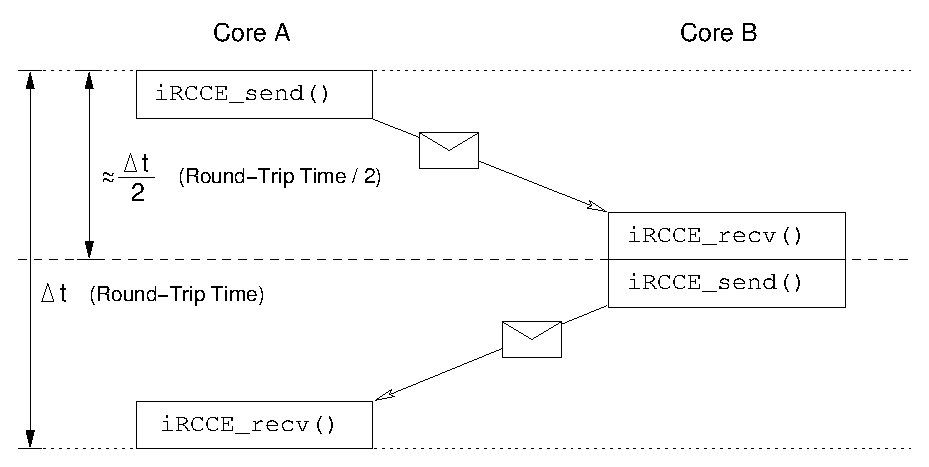
\includegraphics[width=14.0cm]{iRCCE_PingPong.eps}
	\caption{Communication Pattern of the iRCCE \emph{Ping-Pong} Benchmark}
	\label{fig:iRCCE_PingPong}
\end{figure}

{\tiny.}
\vspace{2.0cm}

\begin{figure}[h]
	\centering
		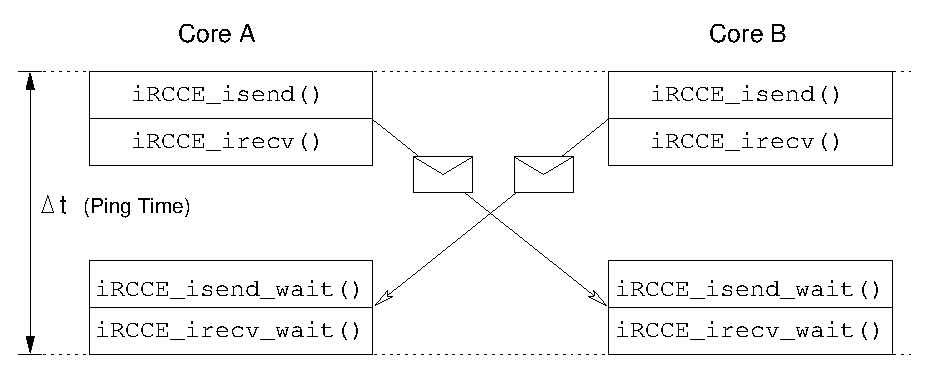
\includegraphics[width=14.0cm]{iRCCE_PingPing.eps}
	\caption{Communication Pattern of the iRCCE \emph{Ping-Ping} Benchmark}
	\label{fig:iRCCE_PingPing}
\end{figure}

\newpage

%******************************************************************************
\section{Non-blocking Communication}\label{sec:communication}
%******************************************************************************

\subsection{Interleaved Communication and Computation}

In many situations, performance can be improved by interleaving communication and computation.
This is particularly true in situations where the communication progress stalls due to a temporary lack of communication resources like intermediate buffers.
In such a situation, a blocking communication function has to wait (either actively by polling or passively by sleeping) until the needed resource becomes available again.
An alternative mechanism in such a situation is to use non-blocking communication functions that do not block but return back to the application immediately if the communication progress can temporarily not be fostered.
Of course, it is up to the application to exploit the interim time until the communication progress can be pushed on again. 
This can be done either by processing computational tasks or by pushing on with other communication requests.
But this in turn means that the application must check repeatedly by itself whether the communication is still stuck or not.
For this purpose, non-blocking communication functions usually pass back a so-call \emph{request handle} which can then be used by additional \emph{push}, \emph{test} or \emph{wait} functions to ensure the communication's progress and eventually its completion.


\subsection{An Exemplary Scenario}

For example, a non-blocking \emph{receive function} will just check if the respective incoming message is already completely available.
If this is not the case (e.g. the sender has not even started the message transfer), the function just records all needed parameters (like the source and the length of the expected message as well as the address of the respective receive buffer) within the request handle and returns it immediately to the application level.
The program can then perform some other application-related calculations, provided that these are independent from the data of the pending message.
However, during these calculations, the program has to call a specific \emph{push function} repeatedly in order to ensure that the communication progress is being fostered in an interleaved manner.
Afterwards, the program has to call an additional \emph{test} or \emph{wait function} in order to check whether the message transfer has been completed.
This approach should be illustrated by the following pseudo-code:

\begin{verbatim}
# Initialize the non-blocking receive request:
CALL non_blocking_receive(OUT request_handle)

# Perform the interleaved computation and communication:
# (the calculation task can be divided into n subtasks)
FOR i = 1 TO n
   CALL partial_calculation(IN i)
   CALL push_communication(VOID)
NEXT i = i + 1

# Ensure that the communication has yet been completed:
CALL wait_for_communication_completion(IN request_handle)
\end{verbatim}

Of course, not only the receiving of a message can be conducted in such a non-blocking and interleaved manner, but also the sending of a message can be processed in a similar way.
The considerations for non-blocking send requests are quite the same as stated above for the receive request and even the programming patterns are quite analogous.
Therefore, we do not present an exemplary non-blocking send scenario at this point.


\subsection{Interleaved vs. Overlapped Communication}

On systems, where the communication can be conducted autonomously by a communication controller (e.g. a DMA engine) or by a communication thread (e.g. on a multi-core CPU), not only an interleaving but rather a true \emph{overlapping} of communication and computation can be achieved.
The main difference between interleaved and overlapped communication is that interleaving implies a concurrent but still serialized processing, whereas a true overlapping results in a parallel processing of communication and computation.
Thus, the first approach helps to hide wait states and to break up message dependencies (see Section \ref{sec:pingping} for an example), but on the other hand it requires an explicit switch-over between computation and communication by frequently calling the push function.
In contrast to this, the second approach can achieve real parallelism and thus does not need an explicit pushing for progress.\footnote{Nevertheless, it should be mentioned that the synchronization between a communication and a computation thread, as well as the latency for setting up a communication controller like a DMA engine, can expose an enormous overhead that can even nullify the performance improvements gained by the parallel progress, especially for short messages.}
However, since there is no other asynchronous hardware (like a communication controller) available for the cores on the SCC, the iRCCE library (currently) just implements the first approach.


\subsection{The Non-Blocking Communication Approach of iRCCE}\label{sec:communication:nonblocking}

As stated above, the iRCCE library implements an interleaving mechanism for non-blocking communication operations.
This is achieved by using the standard RCCE communication functions\footnote{These are the send and receive functions (\texttt{RCCE\_send()}/\texttt{RCCE\_recv()}) of the \emph{non-gory} interface of RCCE.} as a template for their iRCCE counterparts, but instead of waiting for a progress flag\footnote{See the \texttt{RCCE\_wait\_until()} calls of \texttt{RCCE\_send/recv\_general() in RCCE\_send/recv.c}.} to be set, the non-blocking \mbox{iRCCE} functions just test the respective flag\footnote{See the \texttt{iRCCE\_test\_flag()} calls of \texttt{iRCCE\_push\_send/recv\_request() in iRCCE\_isend/irecv.c}.} and return immediately if a progress cannot be made right away.
%
In order to resume the communication late on, the current progress states are stored in request handles that are of type \texttt{iRCCE\_SEND/RECV\_REQUEST}\footnote{These are just C structs that are defined in \texttt{iRCCE.h}}.
These handles are set up and returned by the respective non-blocking send/receive functions (\texttt{iRCCE\_isend()}/\texttt{iRCCE\_irecv()}) that have to be called in order to initiate a non-blocking communication request.
%
Subsequently, the communication progress can be pushed on by calling \texttt{iRCCE\_isend/irecv\_push()} repeatedly.
Again, also these functions return immediately if the communication progress can temporarily not be fostered.
Finally, the completion of a once pending communication request must be ensured by a call to the \texttt{iRCCE\_isend/irecv\_test()} or to the \texttt{iRCCE\_isend/irecv\_wait()} function with the respective request handle as function parameter.

\textbf{Before the completion of a non-blocking operation is not ensured by a call to these functions, neither the respective receive buffer is guaranteed to be valid (it is likely that the message has yet not arrived in the receive buffer) nor the respective send buffer is allowed to be modified (it is likely that the message has yet not been copied out of the send buffer).}

In order to handle multiple outstanding communication requests, the iRCCE library implements a queuing mechanism.
This is necessary, because it is possible to initiate subsequent non-blocking send requests, for example, to the same destination even before the first message gets started to be transferred.
Thus, without a queuing mechanism, the order of the messages could not be observed.
The iRCCE library implements this queuing mechanism in terms of single-linked lists with \emph{one}\footnote{Consequently, send requests (even to different remote ranks) are always processed in the order of their respective \texttt{iRCCE\_isend()} calls; whereas receive requests are handled in the order of the message arrival.} send and 48 receive queues per core.
If the first element in such a list is not \texttt{NULL} (that means that a previous request is still in progress) the new request is just added at the end of the list.
Otherwise, the \texttt{iRCCE\_isend/irecv()} function tries to complete the new request directly.
If such a completion cannot be achieved, the request becomes the head of the respective list and the function returns immediately.

According to this, if one wants to foster the communication progress irrespectively from a specific request, just the \emph{first} pending request in the respective queue needs to be pushed; and that is exactly what \texttt{iRCCE\_isend/irecv\_push()} does.
In contrast to this, \texttt{iRCCE\_isend/irecv\_test()} only checks and pushes that request that is passed as the function argument.
However, these test functions can alternatively be called with \texttt{NULL} as the argument indicating that the respective queue as a whole is meant.
And likewise, when calling \texttt{iRCCE\_isend/irecv\_wait()} with \texttt{NULL} as the argument, the completion of the whole pending queue is waited for.
Furthermore, even \texttt{iRCCE\_isend/irecv()} can be called with \texttt{NULL} as the request argument.
In such a case, a subsequent \texttt{wait()} call will be issued internally.

\subsection{An Example Code: The Ping-Ping Pattern}\label{sec:pingping}

In this section, we want to detail the communication kernel of the Ping-Ping benchmark that is part of the iRCCE distribution (see Section \ref{sec:applications}).
The Ping-Ping pattern (see Figure \ref{fig:iRCCE_PingPing}) is an example for common communication patterns where messages are exchanged in a \emph{symmetric} manner.
In contrast to the notorious Ping-Pong pattern (see Figure \ref{fig:iRCCE_PingPong}), the Ping-Ping pattern is symmetric in this respect that both participating processes do exactly the same: (1) initiate a send request, (2) initiate a receive request and then (3) wait for their completion:

\begin{verbatim}
      iRCCE_SEND_REQUEST send_request;
      iRCCE_RECV_REQUEST recv_request;
      
      char send_buffer[length];
      char recv_buffer[length];
      
      int my_rank     = RCCE_ue();
      int remote_rank = (my_rank + 1) % 2;
      
      RCCE_barrier(&RCCE_COMM_WORLD);
      
        
      timer = RCCE_wtime();
           
      for(round=0; round < numrounds+1; round++)
      {      
         /* (1) send PING via non-blocking send: */
         iRCCE_isend(send_buffer, length, remote_rank, &send_request);

         /* (2) receive PING via non-blocking recv: */
         iRCCE_irecv(recv_buffer, length, remote_rank, &recv_request);
      
         /* (3) wait for completion: */
         iRCCE_isend_wait(&send_request);
         iRCCE_irecv_wait(&recv_request);
      }
       
      timer = RCCE_wtime() - timer;      
\end{verbatim}

\noindent As one can see, without non-blocking communication functions, this pattern could not be realized because the symmetric blocking send calls would both stuck in anticipation of the matching but subsequent receive calls.

\newpage

%******************************************************************************
\section{Extended Range of Functions}\label{sec:extended}
%******************************************************************************

Besides the yet presented iRCCE functions for handling non-blocking communication, we have also added some more higher-level functions for a more convenient handling of outstanding non-blocking requests. This additional part of the iRCCE API should be detailed in this section.


\subsection{Functions for Canceling Requests}\label{sec:extended:cancel}

First of all, we have added functions for canceling already enqueued but not yet started send and receive requests (\texttt{iRCCE\_isend\_cancel()}/\texttt{iRCCE\_irecv\_cancel()}).
By means of these functions, it can be \emph{attempted} to remove such a request from the respective waiting queue until it becomes the head of it.
However, if the request has already become the first and the actual communication has already been started, a subsequent canceling is no longer possible.
In such a case, the cancel function returns the information that the requested withdrawal has failed.
But this in turn means that the started request has to be matched by a respective send or receive call on the remote side.\footnote{This is because otherwise the pending request will wait eternally at the head of the queue and will hinder all following requests from being processed.}
Therefore, the application programmer should be clear in one's mind about the fact that a cancel call may fail and that the application's communication pattern must be designed in such a way that all started non-blocking requests are resolved.

\subsection{Functions for Handling Multiple Outstanding Requests}\label{sec:extended:multiple}

In many cases one wants request some amount of non-blocking send/receive operations, then do calculations in some kind of loop and from time to time test if the send/receive operations have succeeded.
For bigger amounts of messages one will certainly write a loop for testing all those requests. Those loops are an unnecessary and uncomfortable duplication of code, so we wrote functions to handle this in a more elegant manner.
\texttt{iRCCE\_test\_all()} will traverse a linked list of send/receive requests and return success if there have been no pending requests, while \texttt{iRCCE\_wait\_all()} is not returning until there are no pending requests left.
One only have to initialize a data structure of type \texttt{iRCCE\_WAIT\_LIST} and add requests to it first.
Analogous to this, \texttt{iRCCE\_test\_any()}/\texttt{iRCCE\_wait\_any()} can be used for testing or waiting for completion of \emph{any} pending operation in the list.


\subsection{Overview of the Additional iRCCE Functions}
\enlargethispage{0.5cm}
\begin{itemize}
  \item \texttt{int iRCCE\_isend\_cancel(iRCCE\_SEND\_REQUEST*, int*);}
	\item \texttt{int iRCCE\_irecv\_cancel(iRCCE\_RECV\_REQUEST*, int*);}
	\item \texttt{void iRCCE\_init\_wait\_list(iRCCE\_WAIT\_LIST*);}
	\item \texttt{void iRCCE\_add\_to\_wait\_list(iRCCE\_WAIT\_LIST*,iRCCE\_SEND\_REQUEST*,iRCCE\_RECV\_REQUEST*);}
	\item \texttt{int iRCCE\_test\_all(iRCCE\_WAIT\_LIST*, int*);}
	\item \texttt{int iRCCE\_wait\_all(iRCCE\_WAIT\_LIST*);}
	\item \texttt{int iRCCE\_test\_any(iRCCE\_WAIT\_LIST*, iRCCE\_SEND\_REQUEST**, iRCCE\_RECV\_REQUEST**);}
	\item \texttt{int iRCCE\_wait\_any(iRCCE\_WAIT\_LIST*, iRCCE\_SEND\_REQUEST**, iRCCE\_RECV\_REQUEST**);}
\end{itemize}

\newpage

%******************************************************************************
\section{Other Improvements of iRCCE to RCCE}\label{sec:improvements}
%******************************************************************************

\subsection{SCC-optimized Memory Copy Functions}\label{sec:improvements:memcpy}

On the current SCC architecture, a write access does \emph{not} perform a cache line fill even if the cache line is not present (\emph{cache on read not on write}).
Therefore, the core writes in this case directly to the main memory and, of course, this is quite expensive in terms of time.
However, if a present cache line is modified, these changes are are not directly applied to main memory but just to the cache.
Thus, when touching a cache line by a read access before modifying its content, subsequent write accesses to this line do not imply a write through to the main memory.
The following SCC-customized functions copy memory from the on-die buffers (MPB) to an off-die region while pre-fetching the cache lines of the destination:
\texttt{iRCCE\_put()} / \texttt{iRCCE\_memcpy\_put()}.
Therefore, these functions avoid the above mentioned SCC-specific bad behavior of write misses.
In turn, if the destination is located in on-die memory (MPB), classical pre-fetching techniques\footnote{See \texttt{include/scc\_memcpy.h} for more details.} are used by the following functions in order to increase the copy performance:
\texttt{iRCCE\_get()} / \texttt{iRCCE\_memcpy\_get()}.
All these functions are internally used by the iRCCE communication functions; but they can also be utilized outside of the library.


\subsection{Pipelined Send and Receive Functions}\label{sec:improvements:pipeline}

The common RCCE send and receive functions\footnote{as well as the non-blocking and the blocking send and receive functions of iRCCE} use the core-local MPB space for sending messages to remote cores.
As one may know, these local buffers are 8KByte MPB space per core.
If a message to be sent is bigger than the available local MPB space, it must be divided into chunks that are then sent piecewise.
For this purpose, the common RCCE functions determine a chunk size that is equal to the amount of the available local MPB space.
However, when using the whole available local MPB space for one single message chunk, the message transport becomes necessarily a serialized process: (1a) sender puts chunk into the MPB, (1b) sender signalizes the chunk's arrival, (2a) receiver gets chunk from the MPB, (2b) receiver signalizes the chunk's removal (see Figure \ref{fig:iRCCE_Pipeline1}).
This processing scheme must then be performed iteratively until the whole message has been transferred.

Therefore, a smarter approach is not to use the whole local MPB as one big chunk but to divide it into two smaller chunks. This is because in this case sender and receiver can work on the MPB simultaneously in a pipelined and parallelized manner: (1a) sender puts message chunk A into the MPB, (1b) sender signalizes the arrival of chunk A, (2a) sender puts message chunk B into the MPB; and \emph{meanwhile}, the receiver can remove chunk A from the MPB, (2b) sender/receiver signalize the arrival/removal of chunk B/A; and so on (see Figure \ref{fig:iRCCE_Pipeline2}).
The differences between both approaches can be made clear by comparing Figure \ref{fig:iRCCE_Pipeline1} and Figure \ref{fig:iRCCE_Pipeline2}.

This pipelining approach is implemented within iRCCE in terms of the blocking \texttt{iRCCE\_send()} and \texttt{iRCCE\_recv()} functions.
It is important that each call of these functions is matched with a call of its respective counterpart on the remote side. That means that a message that is sent via \texttt{iRCCE\_send()} must necessarily be received via \texttt{iRCCE\_recv()}; and vice versa. This is because the pipelining requires that both the sender and the receiver cooperate \emph{synchronously} according to the pipelining technique.
That this technique can really help to improve the communication performance especially for larger messages can be proved by applying appropriate benchmark tool, as for example shown here in \mbox{Section \ref{sec:performance}}.
However, one should remember that this technique (at least in its current implementation) just takes effect for messages that are bigger than the local MPB space of 8KByte.

\begin{figure}[ht]
	\centering
		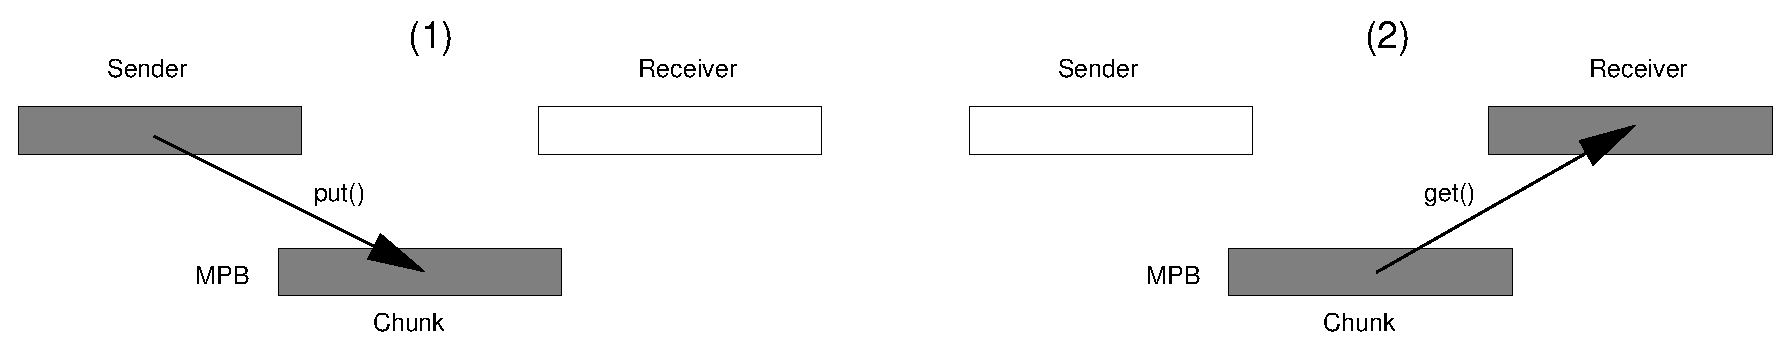
\includegraphics[width=13.0cm]{iRCCE_Pipeline1.eps}
	\caption{Serialized Transport of Message Chunks through the MPB Space}
	\label{fig:iRCCE_Pipeline1}
\end{figure}


\begin{figure}[ht]
  \vspace{0.5cm}
	\centering
		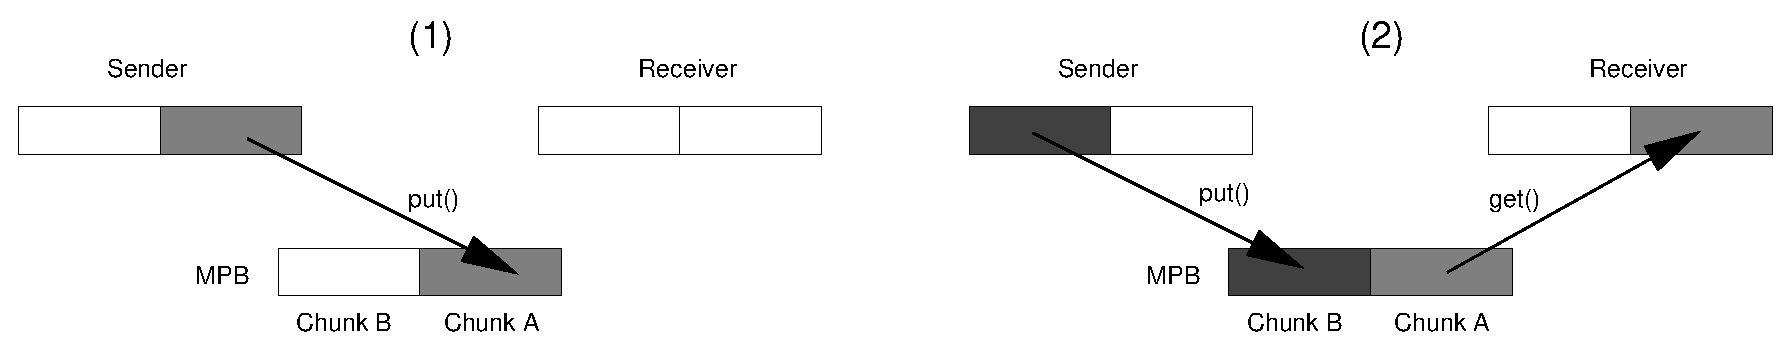
\includegraphics[width=13.0cm]{iRCCE_Pipeline2.eps}
	\caption{Pipelined Transport of Message Chunks through the MPB Space}
	\label{fig:iRCCE_Pipeline2}
	\vspace{0.5cm}
\end{figure}


%******************************************************************************
\section{Known Problems and Issues}\label{sec:problems}
%******************************************************************************

\begin{itemize}

	\item {\sffamily\normalsize\textbf{Differences between MPI and iRCCE Semantics}} \\
Although some function names of iRCCE are quite similar to their counterparts of the Message Passing Interface Standard (MPI) \cite{MPI}, usage and semantics of both APIs differ in detail.
So, for example, the test function of iRCCE only checks and pushes that non-blocking request that is passed via the respective function call.
In contrast to this, the MPI test function also triggers the so-called progress engine that ensures that all waiting requests are checked for progress irrespectively from the passed request of the function call.

	\item{\sffamily\normalsize\textbf{Matching of Non-Blocking Requests with Blocking Function Calls}} \\
Although not extensively tested, a call e.g. of the blocking RCCE send function (\texttt{RCCE\_send()}) should match with a call of its non-blocking iRCCE counterpart (\texttt{iRCCE\_irecv()}) on the remote side; and vice versa.
\emph{But beware!} This is true for matching non-blocking iRCCE calls with blocking RCCE calls, but not for mixing non-blocking calls with the blocking but \emph{pipelined} functions of iRCCE, as for example \texttt{iRCCE\_recv()}.\footnote{This is because the pipelining requires that both the sender and the receiver cooperate \emph{synchronously} according to the pipelining technique (see Section \ref{sec:improvements:pipeline}).}
Moreover, calling a blocking RCCE function after initiating a still pending non-blocking iRCCE function can cause deadlocks because of the missing \texttt{push()} calls!\footnote{Better use \texttt{iRCCE\_isend/irecv()} with \texttt{NULL} as the request argument in this case because the internal \texttt{wait()} call avoids such deadlocks (see Section \ref{sec:communication:nonblocking}).}

	\item {\sffamily\normalsize\textbf{Mixing of Non-Blocking Function Calls with Collective Operations}} \\
Do not use collective communication operations (like \texttt{RCCE\_bcast} or \texttt{RCCE\_barrier}) when there are still outstanding non-blocking communication requests!
This is because since RCCE does not use message tags like MPI, iRCCE cannot distinguish internally between collective and point-to-point requests. 
Thus, an overlapping of non-blocking transfers with collective communication patterns can lead to message mismatches and deadlocks.

\enlargethispage{1.0cm}

	\item {\sffamily\normalsize\textbf{Allocating MPB Space or Flags during Non-Blocking Communication}} \\
Do not allocate new flags or new MPB regions when there are still outstanding non-blocking communication requests!
This is because the amount and the position of the MPB space used for the asynchronous data transfers is recorded at creation time of the respective non-blocking communication request and internally used throughout the request's completion. 

\end{itemize}

%******************************************************************************
\section{Performance Results and Comparisons}\label{sec:performance}
%******************************************************************************

In this section, we want to present some performance results.
In Figure \ref{fig:iRCCE_PingPong_results}, one can see the Ping-Pong bandwidth\footnote{See \cite{ISC2010} for a detailed analysis of the bandwidth curve progression and its correlation with cache level sizes.} (measure with the iRCCE Ping-Pong benchmark, see Section \ref{sec:applications}) for different message sizes and different optimization approaches.
All measurements were done between the cores \texttt{rck00} and \texttt{rck01} with network and memory running at 800MHz and a core frequency of 533MHz (\texttt{Tile533\_Mesh800\_DDR800}).
The used libraries were standard RCCE (V 1.0.13, \texttt{big\_flags}, \texttt{nongory}) and our iRCCE.
%
The figure shows a performance comparison between the \emph{standard RCCE} functions (\texttt{RCCE\_send/recv()}), the utilization of \emph{improved memory copy} functions (\texttt{iRCCE\_memcpy\_put/get()}) and the the applying of \emph{Pipelining} (\texttt{iRCCE\_send/recv()}) for long messages ($length > 8192$).
As one can see, iRCCE outperforms RCCE with respect to the communication bandwidth especially in case of larger messages.
However, the average latency for a 1Byte message still remains the same since the improved memory copy function does not take effect for messages smaller than a cache line.

\begin{figure}[h]
	\centering
	  \vspace{1.5cm}
		\includegraphics[width=14.0cm]{iRCCE_PingPong_results.eps}
	\caption{Some Results of the \emph{iRCCE Ping-Pong} Benchmark: Performance comparison in terms of communication bandwidth between the \emph{standard RCCE} functions (\texttt{RCCE\_send/recv()}), the utilization of \emph{improved Memory-Copy} functions (\texttt{iRCCE\_memcpy\_put/get()}) and the the applying of \emph{Pipelining} (\texttt{iRCCE\_send/recv()}) for long messages ($length > 8192$)}
	\label{fig:iRCCE_PingPong_results}
\end{figure}

\newpage

%******************************************************************************
\section{The iRCCE Application Programming Interface}\label{sec:API}
%******************************************************************************

\setcounter{secnumdepth}{2}% Nummerierung nur bis \subsection 

\subsection{Library Initialization Function}

\subsubsection{int iRCCE\_init(void)}\vspace{-0.3cm}
This function must be invoked before any other iRCCE function is called.
The function initializes crucial data structures of the iRCCE library as for example the queues for pending communication requests. The return value should always be \texttt{iRCCE\_SUCCESS}.


\subsection{Functions for Non-Blocking Sending}

\subsubsection{int iRCCE\_isend(char *buffer, size\_t length, int dest, iRCCE\_SEND\_REQUEST *request)}\vspace{-0.3cm}
This function initiates a request for a non-blocking send operation. The function initializes a request handle of type \texttt{iRCCE\_SEND\_REQUEST} that must be passed as a pointer and that is used later on for checking for the operation's completion.
The function returns \texttt{iRCCE\_SUCCESS} in that case that the request could be finished already within this function call.
However, usually the function returns \texttt{iRCCE\_PENDING} or \texttt{iRCCE\_RESERVED} indicating that the communication has been started but not yet finished or that there are prior requests pending in the send queue and that the request is being reserved.
For more details about this function see Section \ref{sec:communication}.

\begin{tabular}{ll}
\texttt{buffer}  & starting address of the message to be sent \\
\texttt{length}  & length of the outgoing message in bytes \\
\texttt{dest}    & rank (ID) of the target process (UE) \\
\texttt{request} & request handle that is used later on for checking for completion \\
                 & (if set to \texttt{NULL}, a subsequent \texttt{iRCCE\_isend\_wait()} call will be issued internally)
\hspace{2.0cm}
\end{tabular}


\subsubsection{int iRCCE\_isend\_test(iRCCE\_SEND\_REQUEST *request, int *flag)}\vspace{-0.3cm}
This function checks whether an initiated request for a non-blocking send operation is already completed.
The function checks and pushes only that request that is passed as the request handle argument.
However, if \texttt{NULL} is passed as the argument, the function checks for the completion of the whole pending send queue.
The function is non-blocking and the return values and their meanings are the same as for \texttt{iRCCE\_isend()}.
Therefore, the argument \texttt{flag} can also be omitted by passing \texttt{NULL} instead.

\begin{tabular}{ll}
\texttt{request} & request handle returned by \texttt{iRCCE\_isend()} \\
\texttt{flag}    & flag that indicates whether the message has been sent (\texttt{1}) or not (\texttt{0})\\
\hspace{2.0cm}
\end{tabular}


\subsubsection{int iRCCE\_isend\_wait(iRCCE\_SEND\_REQUEST *request)}\vspace{-0.3cm}
This function can be used for waiting for the completion of a pending send request.
Since this function blocks until the respective request is finished, the function also pushes the pending receive queue as well as the pending send requests that are enqueued prior to that request in order to avoid deadlocks.
However, if \texttt{NULL} is passed as the request handle argument, the completion of the whole pending send queue is waited for.
The return value should always be \texttt{iRCCE\_SUCCESS}.

\begin{tabular}{ll}
\texttt{request} & request handle returned by \texttt{iRCCE\_isend()} \\
\hspace{2.0cm}
\end{tabular}


\subsubsection{int iRCCE\_isend\_push(void)}\vspace{-0.3cm}
This function pushes the progress of non-blocking communication requests that are enqueued in the pending send queue.
The function is non-blocking and the return value is \texttt{iRCCE\_PENDING} in case of still pending send requests or \texttt{iRCCE\_SUCCESS} if the send queue is empty.


\subsection{Functions for Non-Blocking Receiving}

\subsubsection{int iRCCE\_irecv(char *buffer, size\_t length, int source, iRCCE\_RECV\_REQUEST *request)}\vspace{-0.3cm}
This function initiates a request for a non-blocking receive operation. The function initializes a request handle of type \texttt{iRCCE\_RECV\_REQUEST} that must be passed as a pointer and that is used later on for checking for the operation's completion.
The function returns \texttt{iRCCE\_SUCCESS} in that case that the request could be finished already within this function call.
However, usually the function returns \texttt{iRCCE\_PENDING} or \texttt{iRCCE\_RESERVED} indicating that the communication has been started but not yet finished or that there are prior requests pending in the receive queue and that the request is being reserved.
For more details about this function see Section \ref{sec:communication}.

\begin{tabular}{ll}
\texttt{buffer}  & starting address of the receive buffer \\
\texttt{length}  & length of the expected message in bytes \\
\texttt{source}  & rank (ID) of the source process (UE) \\
\texttt{request} & request handle (if set to \texttt{NULL}, \texttt{iRCCE\_irecv\_wait()} will be called internally)
\hspace{2.0cm}
\end{tabular}


\subsubsection{int iRCCE\_irecv\_test(iRCCE\_RECV\_REQUEST *request, int *flag)}\vspace{-0.3cm}
This function checks whether an initiated request for a non-blocking receive operation is already completed.
The function checks and pushes only that request that is passed as the request handle argument.
However, if \texttt{NULL} is passed as the argument, the function checks for the completion of the whole pending receive queue.
The function is non-blocking and the return values and their meanings are the same as for \texttt{iRCCE\_irecv()}.
Therefore, the argument \texttt{flag} can also be omitted by passing \texttt{NULL} instead.

\begin{tabular}{ll}
\texttt{request} & request handle returned by \texttt{iRCCE\_irecv()} \\
\texttt{flag}    & flag that indicates whether the message has been received (\texttt{1}) or not (\texttt{0})\\
\hspace{2.0cm}
\end{tabular}


\subsubsection{int iRCCE\_irecv\_wait(iRCCE\_RECV\_REQUEST *request)}\vspace{-0.3cm}
This function can be used for waiting for the completion of a pending receive request.
Since this function blocks until the respective request is finished, the function also pushes the pending send queue as well as the pending receive requests that are enqueued prior to that request in order to avoid deadlocks.
However, if \texttt{NULL} is passed as the request handle argument, the completion of the whole pending receive queue is waited for.
The return value should always be \texttt{iRCCE\_SUCCESS}.

\begin{tabular}{ll}
\texttt{request} & request handle returned by \texttt{iRCCE\_irecv()} \\
\hspace{2.0cm}
\end{tabular}


\subsubsection{int iRCCE\_irecv\_push(void)}\vspace{-0.3cm}
This function pushes the progress of non-blocking communication requests that are enqueued in the pending receive queues.
The function is non-blocking and the return value is \texttt{iRCCE\_PENDING} in case of still pending receive requests or \texttt{iRCCE\_SUCCESS} if the receive queue is empty.

\subsection{Blocking but Pipelined Communication Functions}

\subsubsection{int iRCCE\_send(char *buffer, size\_t length, int dest)}\vspace{-0.3cm}
This function is quite similar to the blocking \texttt{RCCE\_send()} function of RCCE.
The main difference is that this function uses an SCC-optimized memory copy routine and that a pipeline technique for larger messages is used (see also Section \ref{sec:improvements} and Section \ref{sec:performance}).
The threshold value for the message size, when pipelining should take effect, is 8KByte per default and the function call must be matched by a remote call of \texttt{iRCCE\_recv()}.

\begin{tabular}{ll}
\texttt{buffer}  & starting address of the message to be sent \\
\texttt{length}  & length of the outgoing message in bytes \\
\texttt{dest}    & rank (ID) of the target process (UE) \\
\hspace{2.0cm}
\end{tabular}


\subsubsection{int iRCCE\_recv(char *buffer, size\_t length, int source)}\vspace{-0.3cm}
This function is quite similar to the blocking \texttt{RCCE\_recv()} function of RCCE.
The main difference is that this function uses an SCC-optimized memory copy routine and that a pipeline technique for larger messages is used (see also Section \ref{sec:improvements} and Section \ref{sec:performance}).
The threshold value for the message size, when pipelining should take effect, is 8KByte per default and the function call must be matched by a remote call of \texttt{iRCCE\_send()}.

\begin{tabular}{ll}
\texttt{buffer}  & starting address of the receive buffer \\
\texttt{length}  & length of the expected message in bytes \\
\texttt{source}  & rank (ID) of the source process (UE) \\
\hspace{2.0cm}
\end{tabular}


\subsection{SCC-customized Put/Get and Mem-Copy Functions}

\subsubsection{int iRCCE\_put(t\_vcharp target, t\_vcharp source, int size, int rank)}\vspace{-0.3cm}
This is the SCC-optimized version of the \texttt{RCCE\_put()} function (see Section \ref{sec:improvements:memcpy} for more details).
The function copies the contents of the buffer pointed to by \texttt{source} into the MPB location pointed to by \texttt{target}.
The data type \texttt{t\_vcharp} is similar to \texttt{volatile char*} and defined in \texttt{RCCE.h}.

\begin{tabular}{ll}
\texttt{target} & an MPB address that will be converted to the appropriate address on the UE \\
\texttt{source} & start address of the data in private memory of the calling UE \\
\texttt{size}   & size of the data to be put into the MPB in bytes \\
\texttt{rank}   & rank (ID) of the target process (UE) \\
\hspace{2.0cm}
\end{tabular}

\subsubsection{int iRCCE\_get(t\_vcharp target, t\_vcharp source, int size, int rank)}\vspace{-0.3cm}
This is the SCC-optimized version of the \texttt{RCCE\_get()} function (see Section \ref{sec:improvements:memcpy} for more details).
The function copies the contents of the MPB location pointed to by \texttt{source} into the buffer pointed to by \texttt{target}.
The data type \texttt{t\_vcharp} is similar to \texttt{volatile char*} and defined in \texttt{RCCE.h}.

\begin{tabular}{ll}
\texttt{target} & address of the destination buffer in private memory of the calling UE \\
\texttt{source} & an offset that, when combined with the remote rank, points to the source MPB\\
\texttt{size}   & size of the data to be gotten from the MPB in bytes \\
\texttt{rank}   & rank (ID) of the source process (UE) \\
\hspace{2.0cm}
\end{tabular}


\subsubsection{void* iRCCE\_memcpy\_put(void* dest, const void* src, size\_t num)}\vspace{-0.3cm}
This function copies \texttt{num} bytes from memory area \texttt{src} to memory area \texttt{dest} in an SCC-optimized manner (see also Section \ref{sec:improvements:memcpy}).
It can be used instead of the common \texttt{memcpy()} routine of \texttt{<string.h>}.

\begin{tabular}{ll}
\texttt{dest} & start address of the destination memory area \\
\texttt{src}  & start address of the source memory area \\
\texttt{num}  & number of bytes to be copied from source to destination \\
\hspace{2.0cm}
\end{tabular}


\subsubsection{void* iRCCE\_memcpy\_get(void* dest, const void* src, size\_t num)}\vspace{-0.3cm}
This function copies \texttt{num} bytes from memory area \texttt{src} to memory area \texttt{dest} in an SCC-optimized manner (see also Section \ref{sec:improvements:memcpy}).
It can be used instead of the common \texttt{memcpy()} routine of \texttt{<string.h>}.

\begin{tabular}{ll}
\texttt{dest} & start address of the destination memory area \\
\texttt{src}  & start address of the source memory area \\
\texttt{num}  & number of bytes to be copied from source to destination \\
\hspace{2.0cm}
\end{tabular}


\subsection{Cancel Functions for Non-blocking Requests}

\subsubsection{int iRCCE\_isend\_cancel(iRCCE\_SEND\_REQUEST *request, int *flag)}\vspace{-0.3cm}
This function tries to cancel a yet not finished non-blocking send request.
If the request has not yet been started of being processed, the canceling should be successful, otherwise this request can no longer be canceled.
The returned flag value indicates whether the canceling was successful or not.
For more details about this function see Section \ref{sec:extended:cancel}.

\begin{tabular}{ll}
\texttt{request} & request that should be removed from the waiting send request queue \\
\texttt{flag}    & flag that indicates whether the canceling was successful (\texttt{1}) or not (\texttt{0}) \\\\
\hspace{2.0cm}
\end{tabular}


\subsubsection{int iRCCE\_irecv\_cancel(iRCCE\_RECV\_REQUEST *request, int *flag)}\vspace{-0.3cm}
This function tries to cancel a yet not finished non-blocking receive request.
If the request has not yet been started of being processed, the canceling should be successful, otherwise this request can no longer be canceled.
The returned flag value indicates whether the canceling was successful or not.
For more details about this function see Section \ref{sec:extended:cancel}.

\begin{tabular}{ll}
\texttt{request} & request that should be removed from the waiting receive request queue \\
\texttt{flag}    & flag that indicates whether the canceling was successful (\texttt{1}) or not (\texttt{0}) \\
\hspace{2.0cm}
\end{tabular}


\subsection{Functions for Handling Multiple Outstanding Requests}
\enlargethispage{0.3cm}

\subsubsection{void iRCCE\_init\_wait\_list(iRCCE\_WAIT\_LIST* wait\_list)}\vspace{-0.3cm}
This function initializes a wait-list and must be called before adding pending communication requests to the respective wait-list.
A wait-list of type \texttt{iRCCE\_WAIT\_LIST} can handle both send and receive requests.

\begin{tabular}{ll}
\texttt{wait\_list} & a pointer to an object of the opaque iRCCE data type \texttt{iRCCE\_WAIT\_LIST} \\
\hspace{2.0cm}
\end{tabular}


\subsubsection{iRCCE\_add\_to\_wait\_list(iRCCE\_WAIT\_LIST* wait\_list, iRCCE\_SEND\_REQUEST *send\_request, \\ 
\hspace{8.63cm} iRCCE\_RECV\_REQUEST *recv\_request)}\vspace{-0.3cm}
This function adds a pending send and/or receive request to a wait-list that must be initialized before by  \texttt{iRCCE\_init\_wait\_list()}.
Either the send request argument or the receive request argument can be set to \texttt{NULL} if there is not request of the respective type to be added.

\begin{tabular}{ll}
\texttt{wait\_list}     & a pointer to the respective wait-list object \\
\texttt{send\_request}  & a pointer to a pending send request to be added to the wait-list (can be \texttt{NULL}) \\
\texttt{recv\_request}  & a pointer to a pending receive request to be added to the wait-list (can be \texttt{NULL}) \\
\hspace{2.0cm}
\end{tabular}


\subsubsection{iRCCE\_test\_all(iRCCE\_WAIT\_LIST* wait\_list, int *flag)}\vspace{-0.3cm}
This function tests for completion of \emph{all} requests in the passed wait-list.
The flag is set to \texttt{1}, if all respective requests are finished, or to \texttt{0} otherwise.
See Section \ref{sec:extended:multiple} for more details about this function.

\begin{tabular}{ll}
\texttt{wait\_list} & a pointer to the respective wait-list object \\
\texttt{flag}       & flag that indicates whether the wait-list is processed (\texttt{1}) or not (\texttt{0})\\
\hspace{2.0cm}
\end{tabular}


\subsubsection{iRCCE\_wait\_all(iRCCE\_WAIT\_LIST* wait\_list)}\vspace{-0.3cm}
This function just waits for completion of \emph{all} requests in the passed wait-list.
See Section \ref{sec:extended:multiple} for more details about this function.

\begin{tabular}{ll}
\texttt{wait\_list} & a pointer to the respective wait-list object \\
\hspace{2.0cm}
\end{tabular}


\subsubsection{iRCCE\_test\_any(iRCCE\_WAIT\_LIST* wait\_list, iRCCE\_SEND\_REQUEST **send\_request, \\ 
\hspace{7.45cm} iRCCE\_RECV\_REQUEST **recv\_request)}\vspace{-0.3cm}
This function tests for completion of \emph{any} request in the passed wait-list.
It returns a pointer to that finished request or \texttt{NULL} otherwise.
In case of a finished send request, \texttt{send\_request} points to this request and \texttt{recv\_request} is set to \texttt{NULL}; and vice versa in case of a finished receive request.

\begin{tabular}{ll}
\texttt{wait\_list}    & a pointer to the respective wait-list object \\
\texttt{send\_request} & returned pointer to a finished send request (or \texttt{NULL}) \\
\texttt{recv\_request} & returned pointer to a finished receive request (or \texttt{NULL}) \\
\hspace{2.0cm}
\end{tabular}


\subsubsection{iRCCE\_wait\_any(iRCCE\_WAIT\_LIST* wait\_list, iRCCE\_SEND\_REQUEST **send\_request, \\ 
\hspace{7.5cm} iRCCE\_RECV\_REQUEST **recv\_request)}\vspace{-0.3cm}
This function just waits for completion of \emph{any} request in the passed wait-list.
In case of a finished send request, \texttt{send\_request} points to this request and \texttt{recv\_request} is set to \texttt{NULL}; and vice versa in case of a finished receive request.
The rank (ID) of the respective sender/receiver can afterwards be determined via \texttt{send\_request->dest}/\texttt{recv\_request->source}.

\begin{tabular}{ll}
\texttt{wait\_list}    & a pointer to the respective wait-list object \\
\texttt{send\_request} & returned pointer to a finished send request (or \texttt{NULL}) \\
\texttt{recv\_request} & returned pointer to a finished receive request (or \texttt{NULL}) \\
\hspace{2.0cm}
\end{tabular}

\section*{Acknowledgment}
The research and development of the iRCCE library was supported by Intel Corporation.
We would like to thank especially Ulrich Hoffmann, Michael Konow and Michael Riepen of Intel Braunschweig for their help and guidance as well as Carsten Scholtes of the University of Bayreuth for his useful feedback.

\small 
\bibliographystyle{plain}
\bibliography{iRCCE_manual}

\end{document}

